\begin{atiTask}[
  title = Die Identitäten von JACOBI und LAGRANGE
]
Bestätigen Sie jeweils im Indexkalkül
\begin{atiSubtasks}
\item die \textsc{Jacobi}-Identität
\[\vec{a}\times (\vec{b}\times \vec{c})+\vec{c}\times (\vec{a}\times \vec{b})+\vec{b}\times (\vec{c}\times \vec{a})=\vec{0}.
\]
\item die \textsc{Lagrange}-Identität
\[(\vec{a}\times \vec{b})(\vec{c}\times \vec{d})=(\vec{a}\vec{c})(\vec{b}\vec{d})-(\vec{a}\vec{d})(\vec{b}\vec{c}).
\]
\end{atiSubtasks}

\end{atiTask}

\begin{atiSolution}
	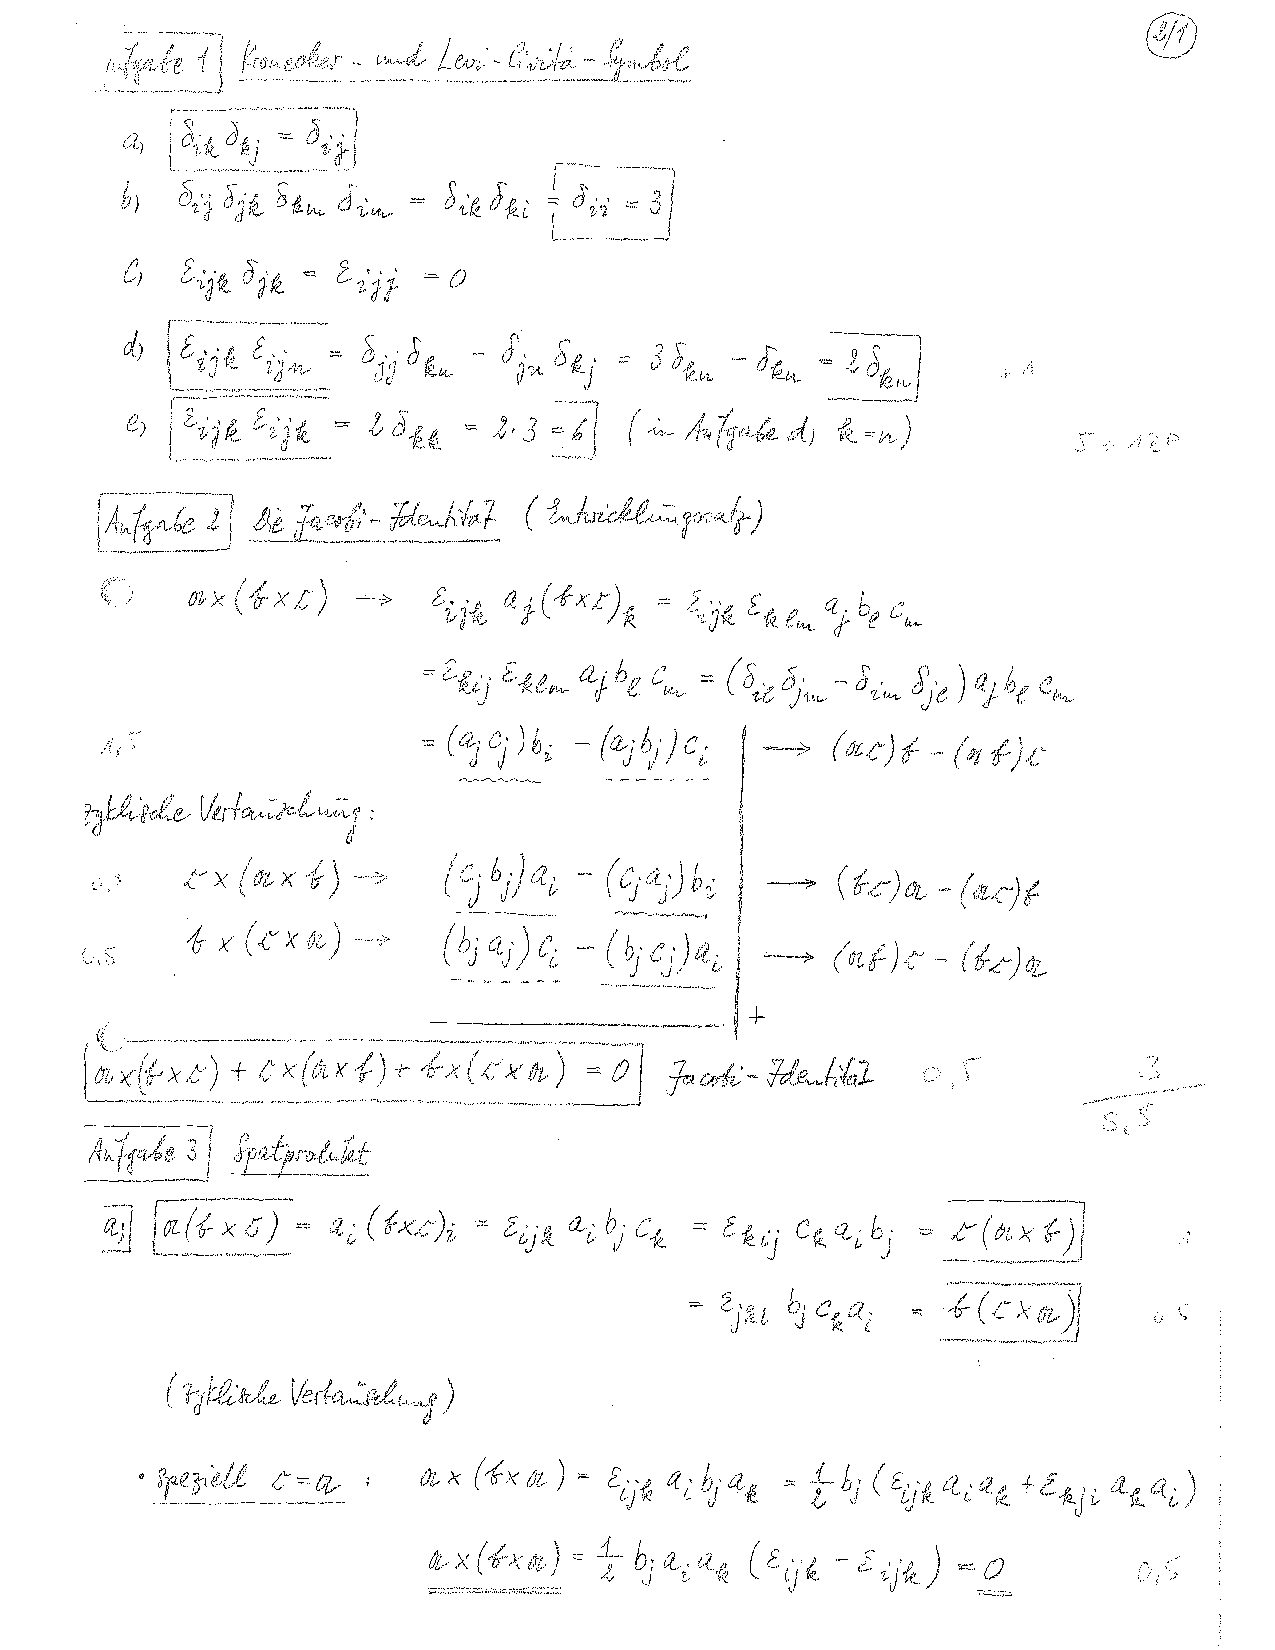
\includepdf[pages=-]{solution-index_iv.pdf}
\end{atiSolution}